
Compressed sensing (CS) has one of the topics that attracted a lot of interests over the past years. Suppose $z$ is a length-$N$ signal. It is said to be $S$-sparse(or compressible) if $z$ can be well approximated using only $S << N$ coefficients under some linear transformation
$ z=\Psi x $
where $\Psi$ is the sparsifying basis and $x$ is transform coefficient vector that has at most $S$(significant) nonzero entries.
\\

The Basis pursuit problem 
\begin{equation}
\min ||x||_{l_1} \quad \text{ subject to } \quad \Phi \Psi x=y
\end{equation}


Where $\Psi$ is an $n \times n$ orthogonal matrix corresponding to the basis in which our signal $z = \Psi x$ is $S$-sparse. $\Phi$ is our sensing matrix. 
\\
\subsection*{Structured matrix}
\textbf{Toeplitz} and \textbf{Circulant} matrices have the forms, respectively,
\\

$$
T = \begin{bmatrix}
t_{1}    & t_{2}    & ...    & t_{n}   \\[0.3em]
t_{n+1}  & t_{1}    & ...    & t_{n-1} \\[0.3em]
\ddots   & \ddots   & \ddots &         \\[0.3em]
t_{2n-1} & t_{2n-2} & ...    & t_{1}         
\end{bmatrix}
\qquad \text{and} \qquad
C = \begin{bmatrix}
t_{1}  & t_{2}  & ...    & t_{n}   \\[0.3em]
t_{n}  & t_{1}  & ...    & t_{n-1} \\[0.3em]
\ddots & \ddots & \ddots &         \\[0.3em]
t_{2}  & t_{3}  & ...    & t_{1}        
\end{bmatrix} 
$$
\\
	Any Circulant matrix can be diagonalized by a Fourier transform, i.e. obeying
	$$ C=\frac{1}{\sqrt{n}} F^* \Sigma F $$ with $F$ as the discrete Fourier matrix
	$F_{t,w}=e^{-i\; 2\pi(t-1)(w-1)/n}, \qquad 1 \le t,w \le n$
	$$
	
	
	\Sigma = \begin{bmatrix}
	\sigma_{1} & 0 & ...& 0           \\[0.3em]
	0 & \sigma_{2} & ... & 0 \\[0.3em]
	\ddots &\ddots & \ddots &      \\[0.3em]
	0 & 0 & ... & \sigma_{n}        
	\end{bmatrix} $$
	a diagonal matrix whose entries are unit magnitude complex numbers with random phases.
\\
	We generate $\sigma_{w}$ as follows:
	\\[1em]
	
	$w=1\qquad \qquad \qquad : \; \sigma_{1} \sim \pm$ 1 with equal probability,
	\\[1em]
	$2 \le w < n/2+1 \; \; : \; \sigma_{w}=e^{i\theta w}, where \; {\theta}_{w} \sim Uniform(0,2\pi) $
	\\[1em]
	$w=n/2+1 \qquad \; \; \, : \; \sigma_{n/2+1} \sim \pm 1 $ with equal probability 
	\\[1em]
	
	$n/2+2 \le w \le n \; \; : \; \sigma_{w}=\sigma^{*}_{n-w+2}$, conjugate of  $\sigma_{n-w+2}$.
	\\
	The construction ensures that $C$ will be orthogonal
	$$ C^*C=\dfrac{{1}}{n} F^* \Sigma F F^* \Sigma F = nI $$
	since $FF^*=F^*F=nI$ and $\Sigma^* \Sigma = I$
	$$
	$$
	Generating the diagonal in this way ensures the resulting circulant matrix is real-valued due to conjugate symmetry.
	$$
	T_{n} = \left[ \: 
	\begin{array}{*{4}{c}}
	\cline{1-4}
	\multicolumn{1}{|c}{t_{1}} & t_{2} & ...& \multicolumn{1}{c|}{t_{n}}           \\[0.3em]
	\cline{1-4}
	t_{n+1} & t_{1} & ... & t_{n-1} \\[0.3em]
	\ddots &\ddots & \ddots &    \\[0.3em]
	t_{2n-1} & t_{2n-2} & ... & t_{1}      \\[0.3em]    
	\end{array}
	\right]
	=
	\left[ \:
	\begin{array}{*{4}{c}}
	t_{1} & t_{2} & ...& t_{n}        \\[0.3em]
	\cline{1-1}
	\multicolumn{1}{|c|}{t_{n+1}} & t_{1} & ... & t_{n-1} \\[0.3em]
	\multicolumn{1}{|c|}{\ddots} & \ddots & \ddots &    \\[0.3em]
	\multicolumn{1}{|c|}{t_{2n-1}} & t_{2n-2} & ... & t_{1}          \\[0.3em]
	\cline{1-1}
	\end{array}
	\right]
	$$
	\\
	$$
	C_{2n} =\begin{bmatrix}
	t_{1}   & t_{2} & ...    & t_{n}  & 0   & t_{2n-1} & ... &  t_{n+1}   \\[0.3em]
	t_{n+1} & t_{1} & ...    & t_{n-1}& ... & 0  & ... &          \\[0.3em]
	\ddots  &       & \ddots &        & \ddots & & &\ddots    \\[0.3em]
	\cdots  &       & \cdots &       & \cdots & & & \cdots
	\end{bmatrix}
	=
	\begin{bmatrix}
	T_{n} & B_{n}            \\[0.3em]
	B_{n} & T_{n}   
	\end{bmatrix}
	$$
	
	\textbf{Hadamard} matrix is a square matrix whose entries are either $+1$ or $-1$ and whose rows are mutually orthogonal.
\begin{figure}[h]
\centering
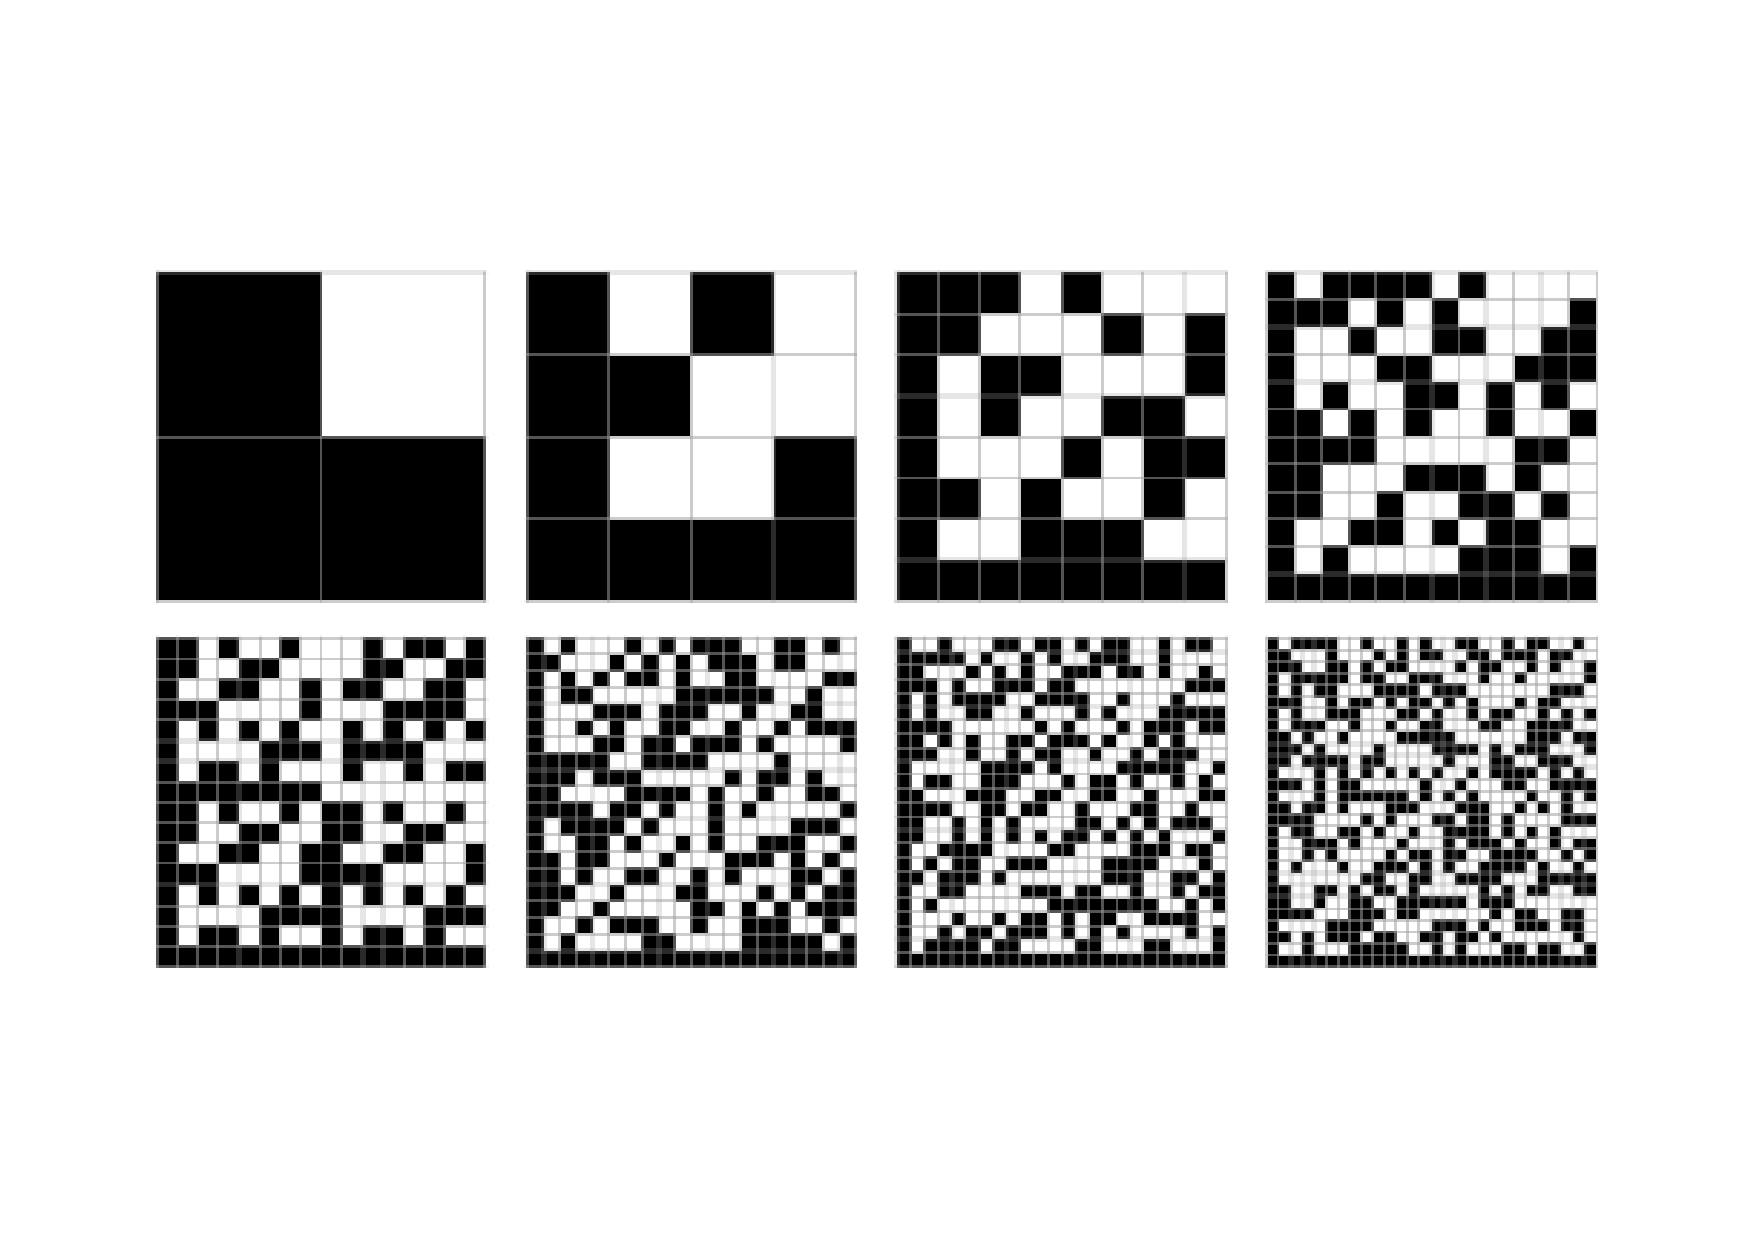
\includegraphics[width=0.7\linewidth]{image/HadamardMatrices_800}
\caption{}
\label{fig:HadamardMatrices_800}
\end{figure}



	An equivalent definition of the Hadamard matrices is given by 
	$$ H_{n} H_{n}^T = n  I_{n} $$
	where $I_{n}$ is the $n \times n$ identity matrix.
	$$
	H_{1} = \begin{bmatrix}
	1
	\end{bmatrix}
	\qquad
	H_{2} = \begin{bmatrix}
	1 & 1           \\[0.3em]
	1& -1
	\end{bmatrix}	
	\qquad
	H_{4} = \begin{bmatrix}
	H_{2} & H_{2}           \\[0.3em]
	H_{2}& -H_{2}
	\end{bmatrix}	
	$$
	$$
	\centering
	\qquad
	H_{2^{n}} = \begin{bmatrix}
	H_{2^{n-1}} & H_{2^{n-1}}           \\[0.3em]
	H_{2^{n-1}}& -H_{2^{n-1}}            
	\end{bmatrix}	
	$$




 
While kernel SVMs have strong theoretical foundations, traditional solvers are too slow in practice and a need for more efficient solvers has arisen given the rapid increases in dataset size in the recent past. With increasing proliferation of multicore processors, techniques for parallelizing SVM computation across cores have become more important. Parallel approaches are particularly important for very large datasets where one machine may not be able to store all the data. In addition, it has been argued~\cite{brugger2006parallel} that subsampling is not sufficient for kernel SVMs where every point may end up being a support vector. A recent paper by \cite{hsieh2013divide} studied clustering based decomposition approaches for large datasets and proposed Divide and Conquer-SVM (DC-SVM) algorithm. It reduced computation time by solving subproblems on portions of the data identified by k-means clustering, and using these solutions to initialize the full problem. They recurse this algorithm over each subproblem to further speed up computation. 
=======
Kernel methods have emerged as a powerful technique for a variety of machine learning tasks. 
Support vector machines for the binary classification problem in particular have been studied in great detail and methods for solving them are well understood. 
>>>>>>> a84b37d29f3107229ab96e8f137ac3bb2a912fb4

The initial goal of this research project was to implement this algorithm using Galois and explore the potential for parallelization. 
DC-SVM involves three steps, all of which can be parallelized: clustering, solving the smaller SVM problems, and concatenating the solutions and solving the full SVM problem with this initialization with dual coordinate descent. 
We will not address the first of these and the second is fairly straightforward but the final solve is most interesting, and our proposed algorithm will use the Galois framework to parallelize this step. As in DC-SVM, we will solve the problem via dual coordinate descent~(CD). Each step of the CD algorithm involves using dual variable values for all other points and thus the updates are all dependent and cannot be parallelized directly. However, in Theorem, we give a simple condition under which \emph{approximate serializability} holds, namely that the points should have sufficiently low kernel similarity. Galois can then be used to select dual coordinates which can be optimized in parallel. Galois supports priority scheduling and we also propose a scheduling algorithm for kernel SVM in this report. As our next step, we are implementing this algorithm in Galois and will run empirical tests on standard datasets to assess potential speedups.

\subsection{Notation and background}
Binary SVMs are defined by the following quadratic optimization problem 
\begin{equation}
	\text{argmin } \frac{1}{2} ||w||_2^2 + C \sum_{i=1}{n} \xi_i
	\label{primal}
\end{equation}
\begin{equation}
	\text{subject to } y_i(w^T x_i - b) \geq 1 \,\,\,\,\, \forall i
	\label{primal_constraint}
\end{equation}

For kernel SVMs, we replace each dot product $ x^T y $ with a kernel function $k_{\sigma}(x,y)$. 
A commonly used kernel is the Gaussian or radial basis function (rbf) kernel, where we use $\sigma$ to denote the bandwidth of the kernel.
\[
	K_{ij} = k_{\sigma}(x_i,x_j) = \exp \left(-\frac{||x_i - x_j||^2_2}{2 \sigma^2}\right)
\]

We will solve the kernel SVM dual problem for $\al$, which can be formulated as follows:
\begin{equation}
	\text{argmin } \frac{1}{2} \al^T Q \al - \bs{1}^T \al
	\label{dual}
\end{equation}
\begin{equation}
	\text{subject to } 0 \leq \al_i \leq C \,\,\,\,\, \forall i
	\label{dual_constraint}
\end{equation}
$C$ is defined as in (\ref{primal}), while $Q$ is defined so $Q_{ij} = y_i y_j K(x_i,x_j)$.

